\section{Dasar Teori}
Subbab dasar teori merupakan subbab yang akan memberikan pengenalan
terhadap permasalahan yang akan dihadapi. Subbab ini juga akan memberikan konteks dan keterangan lebih lanjut mengenai teknologi-teknologi yang akan digunakan atau dipertimbangkan sebagai alternatif solusi dari permasalahan yang diangkat. Berikut merupakan landasan teori yang akan digunakan dalam penelitian ini.

\subsection{Pemrosesan Dokumen Finansial}
\label{subsec:pemrosesan-dokumen-finansial}

Dokumen struk pembayaran memegang peranan penting dalam pengelolaan
keuangan baik individu maupun institusi. Proses ekstraksi data dari dokumen-dokumen ini sering kali menghadapi tantangan yang signifikan, termasuk keanekaragaman tata letak, kualitas gambar yang bervariasi, dan kebutuhan untuk
mengekstrak informasi dengan akurasi tinggi. Sebagai contoh, elemen-elemen penting seperti total harga, tanggal transaksi, dan nomor rekening sering kali tersebar di berbagai posisi dalam dokumen yang berbeda, sehingga membuat ekstraksi data secara manual menjadi lambat dan rentan terhadap kesalahan.

Teknologi yang umumnya dapat digunakan untuk menanggulangi masalah ini adalah \cv{}, salah satunya \ocr. Secara tradisional, \ocr{} digunakan untuk mengonversi teks dalam gambar menjadi format digital yang dapat diproses lebih lanjut. Namun, OCR memiliki
keterbatasan, terutama dalam menangani dokumen dengan kualitas gambar rendah atau format teks yang tidak standar. Selain itu, ketergantungan pada OCR dapat meningkatkan kompleksitas dan biaya pemrosesan \parencite{kim2021donut}.

\dlfl{} memiliki berbagai jenis algoritma dan model yang mendukung pengembangan sistem tersebut. \dl{} merupakan cabang \ml{} yang memanfaatkan jaringan saraf tiruan berlapis untuk mengenali pola kompleks dalam data, termasuk dokumen finansial. Salah satu model yang umum digunakan adalah \cnn. \cnn{} dirancang untuk memproses data berbentuk gambar dengan mendeteksi fitur lokal seperti teks, garis, atau elemen visual lainnya sehingga \linebreak cocok untuk ekstraksi data dari dokumen. Namun, \cnn{} terbatas dalam memahami hubungan global antar
elemen dalam dokumen sehingga \transformer{} hadir sebagai solusi yang lebih canggih \parencite{alzubaidi2021review}.

Dengan mekanisme \attention-nya, \transformer{}, seperti LayoutLM dan
Donut, mampu menangkap hubungan kontekstual antar elemen secara global. Hal ini membuat penggunaan \transformer{} dengan struktur kompleks dan informasi
tersebar. \transformer{} memberikan pendekatan yang kuat untuk memastikan akurasi dan efisiensi dalam pemrosesan dokumen finansial.

\subsection{\emph{Deep Learning}}
\label{subsec:dl}

\dlfl{} adalah cabang dari \ml{} yang menggunakan \annfull{} dengan banyak lapisan untuk mempelajari representasi data yang kompleks. Deep Learning memungkinkan komputer untuk menganalisis data tidak terstruktur, seperti teks, gambar, audio, dan video dengan tingkat akurasi yang sangat tinggi. Model-model \dl{} belajar dengan cara memproses data melalui lapisan-lapisan neuron atau saraf yang dirancang untuk mengekstrak fitur-fitur penting, baik yang eksplisit maupun tersembunyi \parencite{Goodfellow-et-al-2016}. 

Terdapat beberapa model dan arsitektur yang dapat digunakan dalam \dl. Setiap model tersebut ditujukan untuk memenuhi kasus yang berbeda-beda. Berikut adalah arsitektur dan model yang relevan dengan kasus ekstraksi data dari dokumen finansial.

\subsubsection {\cnn\--\transformer{}}
\cnn{} dan \transformer{} adalah dua metode yang dapat digunakan secara terpisah atau bersama untuk menangani data visual. \cnn{} adalah salah satu jenis \MakeLowercase{{\nn{}}} yang sering digunakan pada data gambar. CNN bisa digunakan untuk mendeteksi dan mengenali fitur signifikan tanpa supervisi manusia pada gambar \parencite{alzubaidi2021review}. \transformer{} adalah sebuah arsitektur \MakeLowercase{\nn{}} yang meng-\emph{encode} data menjadi fitur-fitur melalui mekanisme \attention. \transformer{} membagi gambar menjadi beberapa \patch{} dan mengkalkulasi representasi hubungan antar \patch{} tersebut \parencite{han2021transformer}. 

\subsubsection{\crnnfull}
\crnn{} adalah kombinasi dari \cnn{} dan \rnn{} yang merupakan dua model yang paling sering digunakan. \cnn{} digunakan pada tahap awal untuk mengekstrak fitur visual dan gambar. Hasil dari implementasi \cnn{} akan digunakan oleh model \rnn{} sebagai data input untuk menangkap hubungan antar elemen teks, seperti urutan huruf dalam kata atau angka dalam bilangan \parencite{wang2019convolutional}. \crnn{} telah diaplikasikan pada klasifikasi musik, audio, dan klasifikasi data serta teks yang bersifat \emph{hyperspectral}.

\subsubsection{Model \objectdetection}
Model \objectdetection{} adalah salah satu model dalam \dl{} yang digunakan untuk mendeteksi dan mengenali objek-objek tertentu dalam sebuah gambar atau dokumen, termasuk elemen-elemen seperti teks, tabel, atau simbol pada dokumen finansial. Dua jenis utama model \objectdetection{} yang sering digunakan adalah \yolofull{} dan \rcnnfull{}.
	\begin{enumerate}
		\item \yolo~\\
		\yolo{} adalah model \objectdetection{} yang dirancang untuk kecepatan tinggi dan efisiensi. \yolo{} memproses seluruh gambar dalam satu tahap dengan membagi gambar menjadi \grid{}, kemudian memprediksi bounding box dan kelas objek secara bersamaan di setiap \grid{} \parencite{diwan2023object}. Model ini terkenal karena kecepatannya. Dengan kecepatan tersebut, model ini cocok untuk aplikasi \emph{real-time} meskipun memiliki kompromi dalam akurasi untuk objek kecil atau yang saling berdekatan.
		\item \rcnn~\\
		\rcnn{} menggunakan pendekatan dua tahap. \rcnn{} menghasilkan proposal wilayah yang berpotensi mengandung objek pada tahap pertama. Pada tahap kedua, setiap proposal dianalisis lebih mendalam menggunakan \cnn{} untuk mengklasifikasikan objek dan memperbaiki bounding box. \rcnn{} dan variannya, yaitu Fast \rcnn{} dan Faster \rcnn{}, menawarkan akurasi tinggi walaupun memerlukan waktu komputasi yang lebih lama. Dengan sifat tersebut, model ini lebih cocok untuk aplikasi yang tidak membutuhkan deteksi \emph{real-time} \parencite{xie2021oriented}.
	\end{enumerate}

\subsection{\transformer}
\label{subsec:transformer}

\transformer{} adalah suatu jenis arsitektur jarigan yang baru dalam \dl. Arsitektur ini digunakan untuk mentransformasi sebuah deretan data menjadi sesuatu dengan karakteristik, seperti panjang atau format, yang berbeda. \transformer{} tidak menggunakan lapisan rekursif (\rnn) atau konvolusi (\cnn). \transformer{} menggunakan mekanisme \selfattention{} yang memungkinkannya untuk memahami hubungan antar elemen dalam sebuah deretan atau urutan (\sequence). Tidak seperti pada \rnn{}, mekanisme \selfattention{} tidak perlu memperhatikan jarak antar elemen. Mekanisme ini membuat \transformer{} menjadi sangat efisien untuk memproses data sekuensial. \transformer{} banyak digunakan pada proses penerjemahan bahasa, rangkuman teks, dan pengenalan suara.

\transformer{} terdiri atas dua komponen utama, yaitu \encoder{} dan \decoder. \encoderfl{} bertugas untuk membaca dan memproses \sequence{} masukan, sementara \decoder{} menghasilkan \sequence{} keluaran berdasarkan informasi dari \encoder. \encoderfl{} dan \decoder{} terdiri dari beberapa lapisan yang identik, dengan masing-masing memiliki dua sub-lapisan utama, yaitu \emph{multi-head attention} dan \emph{feed-forward network}.

\subsubsection{\mha}
Sublapisan ini menggunakan mekanisme \selfattention{} untuk memahami hubungan antar elemen dalam sebuah \sequence{}. Misalnya, dalam sebuah kalimat, mekanisme ini dapat mengenali bahwa kata "dia" merujuk pada "ibu" meskipun terdapat kata-kata lain di antaranya. \mha{} merupakan gabungan beberapa lapisan (\layer) \emph{Scaled Dot-Product Attention}, atau akan disingkat menjadi \attention. Perbandingan proses pada \mha{} dan \emph{Scaled Dot-Product Attention} dapat dilihat pada \autoref{fig:attention}
	\begin{figure}[htbp]
		\centering
		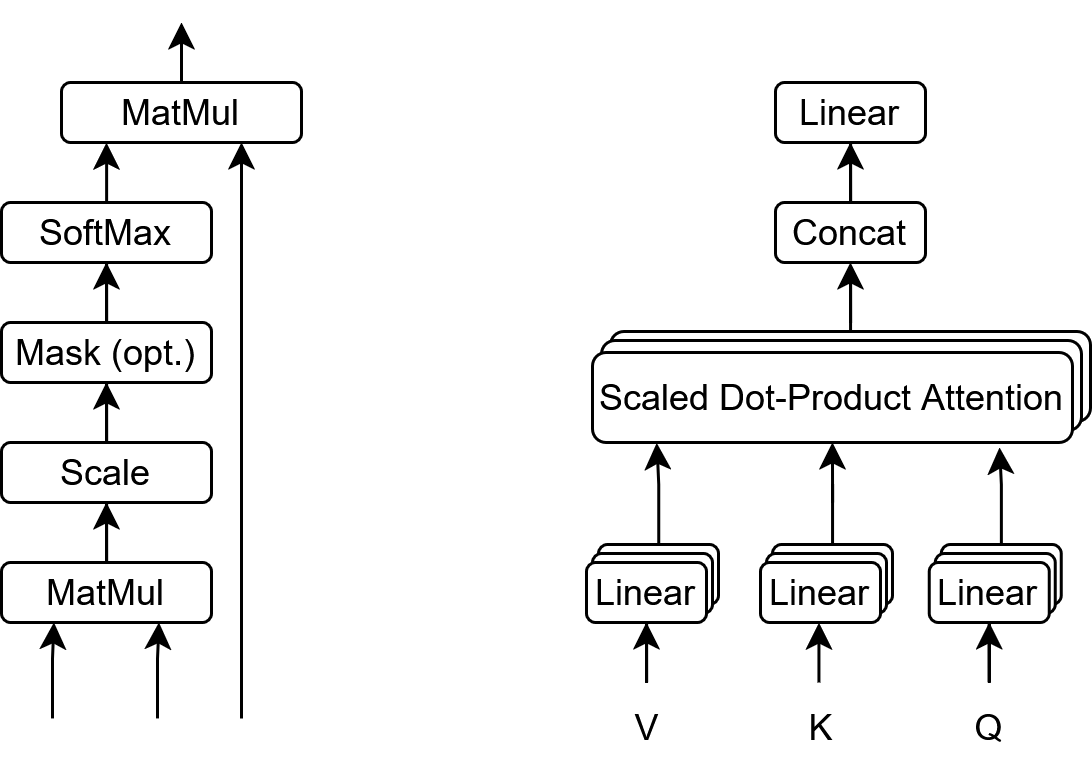
\includegraphics[width=.8\textwidth]{images/attentionmha.png}
		\caption{\emph{Scaled Dot-Product Attention} (kiri) dan \mha{} (kanan) yang merupakan beberapa \layer{} \attention{} berjalan paralel \parencite{vaswani2017attention}}
		\label{fig:attention}
	\end{figure}

$Q$ (\emph{Query}), $K$ (\emph{Key}), dan $V$ (\emph{Value}) adalah representasi vektor dari setiap elemen dalam sebuah \sequence. Simbol $d_k$ adalah dimensi dari vektor $K$ yang digunakan untuk menghasilkan perkalian \emph{dot-product} $QK^\mathsf{T}$ agar proses pelatihan tetap stabil. Fungsi Softmax kemudian mengubah skor tersebut menjadi bobot probabilistik untuk menentukan elemen yang paling relevan untuk diperhatikan.
\newpage
Perhitungan \attention{} dilakukan dengan formula seperti yang ditunjukkan pada persamaan \eqref{eq:attention-softmax} \parencite{vaswani2017attention} yang didefinisikan sebagai berikut.

\begin{equation}
	\label{eq:attention-softmax}
		\operatorname{Attention}(Q, K, V) = \operatorname{SoftMax}\left(\frac{QK^\mathsf{T}}{\sqrt{d_k}}\right)V
\end{equation}
\addcontentsline{loe}{myequations}{\protect\numberline{\theequation}Persamaan Softmax}

\subsubsection{\ffnfull}
Setelah \attention{} dihitung, informasi dari setiap elemen diproses melalui jaringan \emph{feed-forward} yang sama untuk setiap posisi dalam \sequence. Jaringan ini terdiri dari dua lapisan linier dengan fungsi aktivasi ReLU pada persamaan \eqref{eq:ffn} \parencite{vaswani2017attention}:

\begin{equation}
	\label{eq:ffn}
	\operatorname{FFN}(x) = \max(0, xW_1 + b_1)W_2 + b_2
\end{equation}
\addcontentsline{loe}{myequations}{\protect\numberline{\theequation}Fungsi Aktivasi ReLU pada \ffn}

\decoderfl{} memiliki perbedaan signifikan dibandingkan dengan \encoder. \encoderfl{} terdiri dari beberapa lapisan yang masing-masing memiliki mekanisme \selfattention{} dan FFN. Setiap elemen dalam \sequence{} dapat saling “memperhatikan”. \decoderfl{} memiliki lapisan tambahan, yaitu \encoder{}\--\decoder{} \attention. Lapisan ini memungkinkan \decoder{} untuk "memperhatikan" keluaran dari \encoder. \decoderfl{} memiliki mekanisme \emph{masking} untuk memastikan bahwa posisi saat ini hanya bergantung pada posisi sebelumnya.

\transformer{} memiliki keunggulan dibandingkan dengan metode konvensional pemrosesan sekuensial, seperti \rnn. \transformer{} tidak bergantung pada pemrosesan berurutan. \transformer{} dapat memproses seluruh urutan secara bersamaan dan membuat pelatihan jauh lebih cepat. Implementasi \transformer{} menunjukkan hasil terbaik di berbagai kasus dibandingkan dengan arsitektur lainnya.


\subsection{\donutfull}
\label{subsec:donut}

\donut{} adalah sebuah transformer yang tidak memerlukan penggunaan \ocr{} untuk melakukan pemahaman terhadap dokumen. Konsep utama \donut{} adalah pemetaan langsung dari gambar dokumen mentah menjadi hasil yang terstruktur dan melewati seluruh proses implementasi \ocr \parencite{kim2021donut}. \donut{} merupakan sebuah \emph{pre-trained model} yang menggunakan \emph{visual encoder Transformer}, yaitu \swin{} untuk melakukan ekstraksi fitur visual dari dokumen, dan \emph{text decoder Transformer}, yaitu \bartfull. Oleh karena itu, \donut{} tidak memiliki ketergantungan pada fungsionalitas \ocr{} sama sekali.

\textit{Pipeline} implementasi \transformer untuk pemahaman dokumen pada umumnya terlihat pada \autoref{fig:non-donut-pipeline}. \donut{} menyederhanakan pipeline ekstraksi data dokumen seperti terlihat pada \autoref{fig:donut-pipeline}. Dengan implementasi \textit{pipeline} yang lebih sederhana, proses ekstraksi data dokumen dapat diproses secara \ee{} melalui Donut tanpa perlu melewati fase \textit{pre-processing} dan \textit{post-processing} dari gambar \textit{input} dan \textit{output}.

\textit{Input} gambar akan diterima oleh \encoder, seperti \swin{} atau ResNet yang akan memecah gambar menjadi gambar-gambar kecil yang tidak saling bertumpuk. Hasil dari \encoder{} akan dikirimkan ke \decoder{} \transformer{} yang digunakan, seperti BART, untuk diproses menjadi \textit{output} berbentuk deretan teks. \textit{Output} yang dihasilkan akan dikonversi menjadi format \jsonfull.

\begin{figure}[htbp]
	\centering
	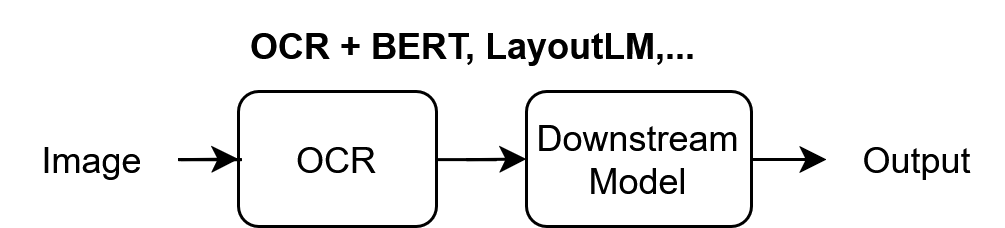
\includegraphics[width=0.8\textwidth]{images/non-donut-pipeline}
	\caption{\textit{Pipeline} sebelum implementasi \donut{} \parencite{kim2021donut}.}
	\label{fig:non-donut-pipeline}
\end{figure}

\begin{figure}[htbp]
	\centering
	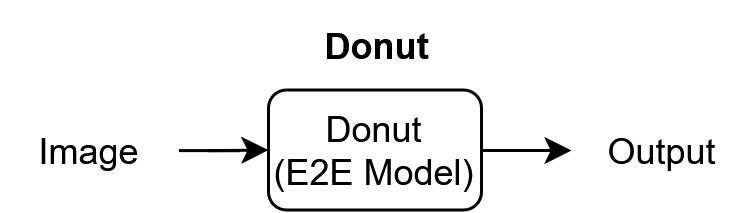
\includegraphics[width=0.8\textwidth]{images/donut-pipeline.png}
	\caption{\textit{Pipeline} setelah implementasi \donut{} \parencite{kim2021donut}.}
	\label{fig:donut-pipeline}
\end{figure}

\subsection{\swin}
\label{subsec:swin}

\swin{} adalah sebuah arsitektur \vitfull{} yang dirancang sebagai penopang dalam berbagai tugas \cv{} seperti klasifikasi gambar, deteksi objek, dan segmentasi semantik. Nama "Swin" berasal dari konsep
"\emph{Shifted Window}" yang menjadi elemen utama dalam desainnya. Tidak seperti \vit{} yang menggunakan metode \selfattention{} secara global
pada seluruh gambar, \swin{} memperkenalkan \selfattention{} berbasis \emph{local window} yang secara signifikan mengurangi kompleksitas komputasi \parencite{liu2021swin}. Perbedaan pendekatan \swin{} dan \vit{} dapat dilihat pada \autoref{fig:Swin-vs-ViT}. 

\begin{figure}[htbp]
    \centering
    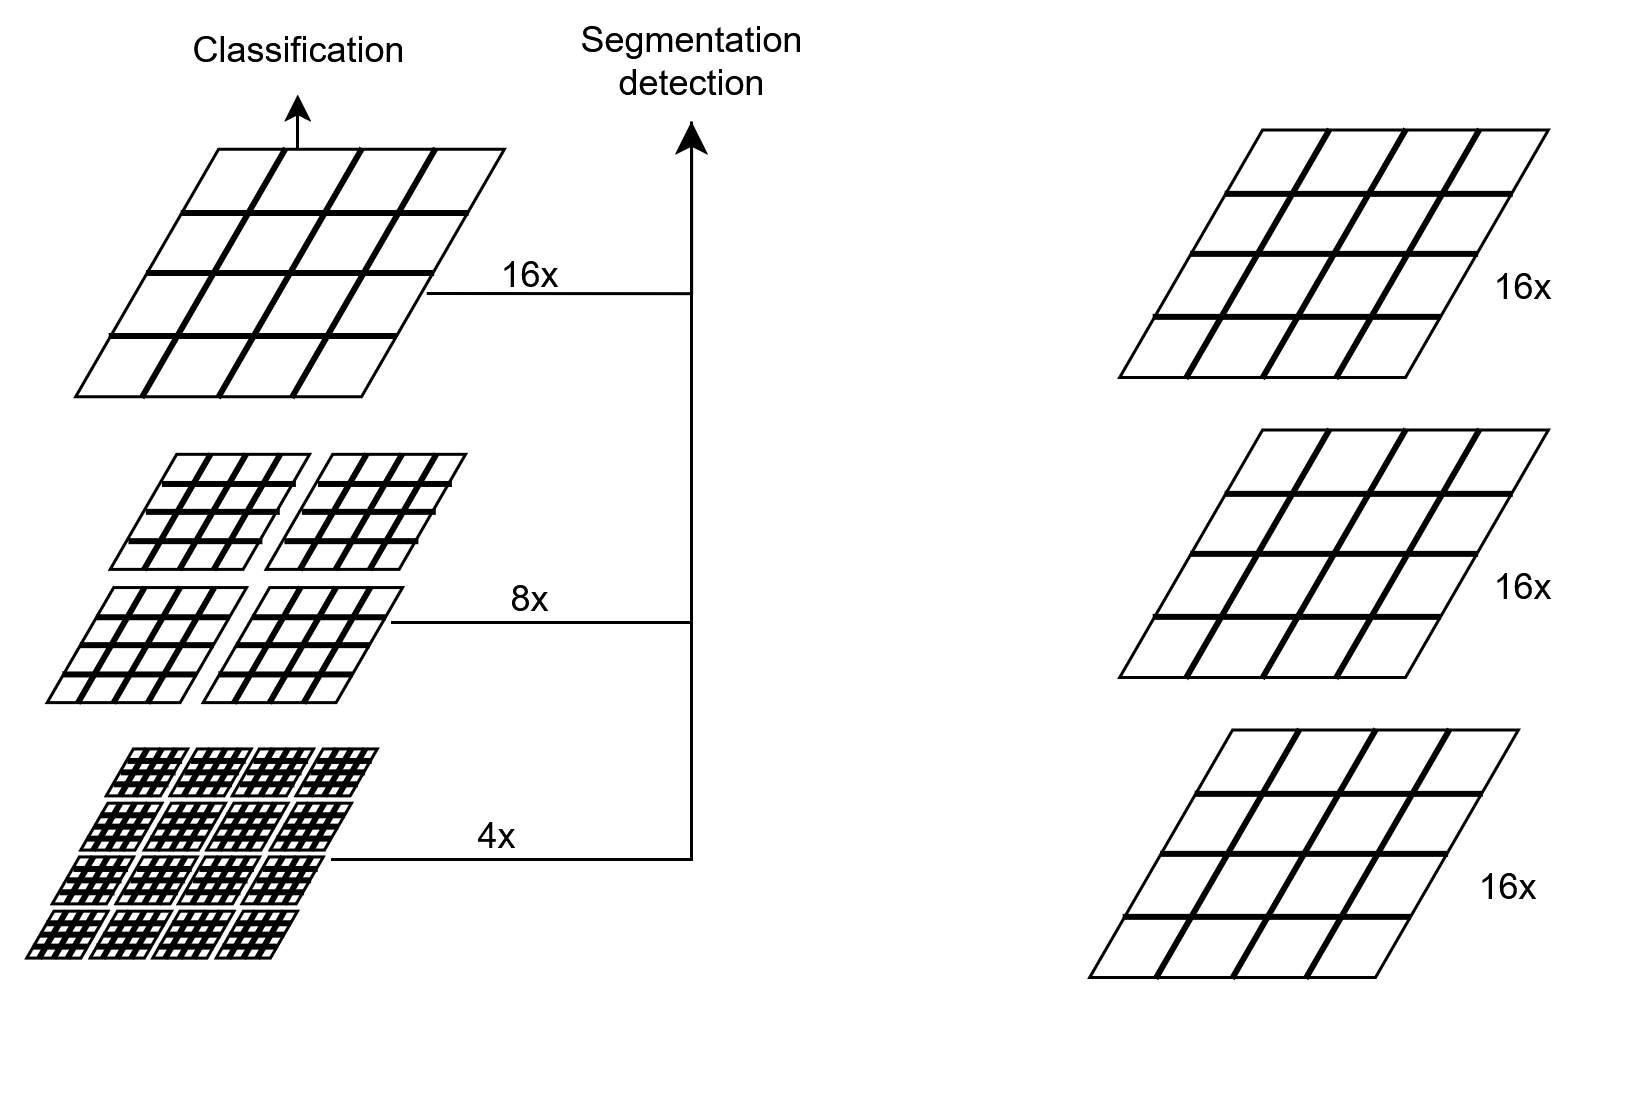
\includegraphics[width=0.8\textwidth]{images/swin-vit.png}
    \caption{Perbandingan antara \swin{} dan \vitfull{} \parencite{liu2021swin}.}
    \label{fig:Swin-vs-ViT}
\end{figure}


\autoref{fig:Swin-shifted-window} menujukkan pendekatan \shiftedwindow{} pada \swin. Selain itu, \swin{} mengadopsi arsitektur hierarkis yang mirip dengan \cnn. Arsitektur ini memungkinkan ekstraksi fitur pada berbagai skala dan menjadikannya lebih efisien dan fleksibel untuk menangani gambar resolusi tinggi dan berbagai tugas prediksi.

\begin{figure}[htbp]
    \centering
    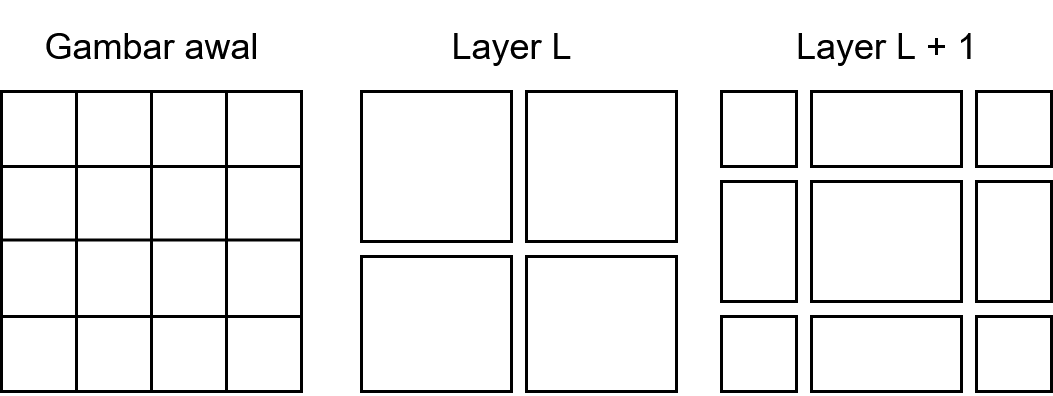
\includegraphics[width=0.7\textwidth]{images/swin-shifted-window.png}
    \caption{Pendekatan \shiftedwindow{} pada \swin{} \parencite{liu2021swin}.}
    \label{fig:Swin-shifted-window}
\end{figure}

Pada \swin, terdapat empat tahap. Pada setiap tahap, resolusi fitur akan secara bertahap dikurangi saat melalui lapisan \emph{patch merging} seperti pada \autoref{fig:swin-architecture}. Contohnya pada tahap satu, resolusi gambar $\frac{H}{4} \times \frac{W}{4}$ dengan dimensi fitur awal C. Kemudian pada tahap dua, resolusi dikurangi menjadi $\frac{H}{8} \times \frac{W}{8}$ dan 
dimensi fitur dinaikkan menjadi 2C. Tahap ini akan berlanjut hingga pada tahap empat dengan resolusi $\frac{H}{32} \times \frac{W}{32}$ dan dimensi 8C. Dengan struktur ini, \swin{} mampu menangkap informasi pada berbagai skala, seperti fitur lokal 
dan global, yang sangat penting dalam \emph{computer vision} seperti \emph{object detection}. 

\autoref{fig:swin-architecture} menunjukkan arsitektur dan cara kerja \swin. Gambar yang masuk dengan dimensi $H \times W$ akan dikonversi menjadi beberapa patch atau potongan kecil $4 \times 4$ pixel. Setiap \patch{} ini kemudian dianggap sebagai token, dan fitur awalnya direpresentasikan oleh nilai RGB-nya. Fitur ini kemudian 
diproyeksikan ke dimensi tertentu C melalui lapisan \emph{embedding} linier seperti yang ditunjukkan pada \autoref{fig:swin-architecture}.

\begin{figure}[htbp]
    \centering
    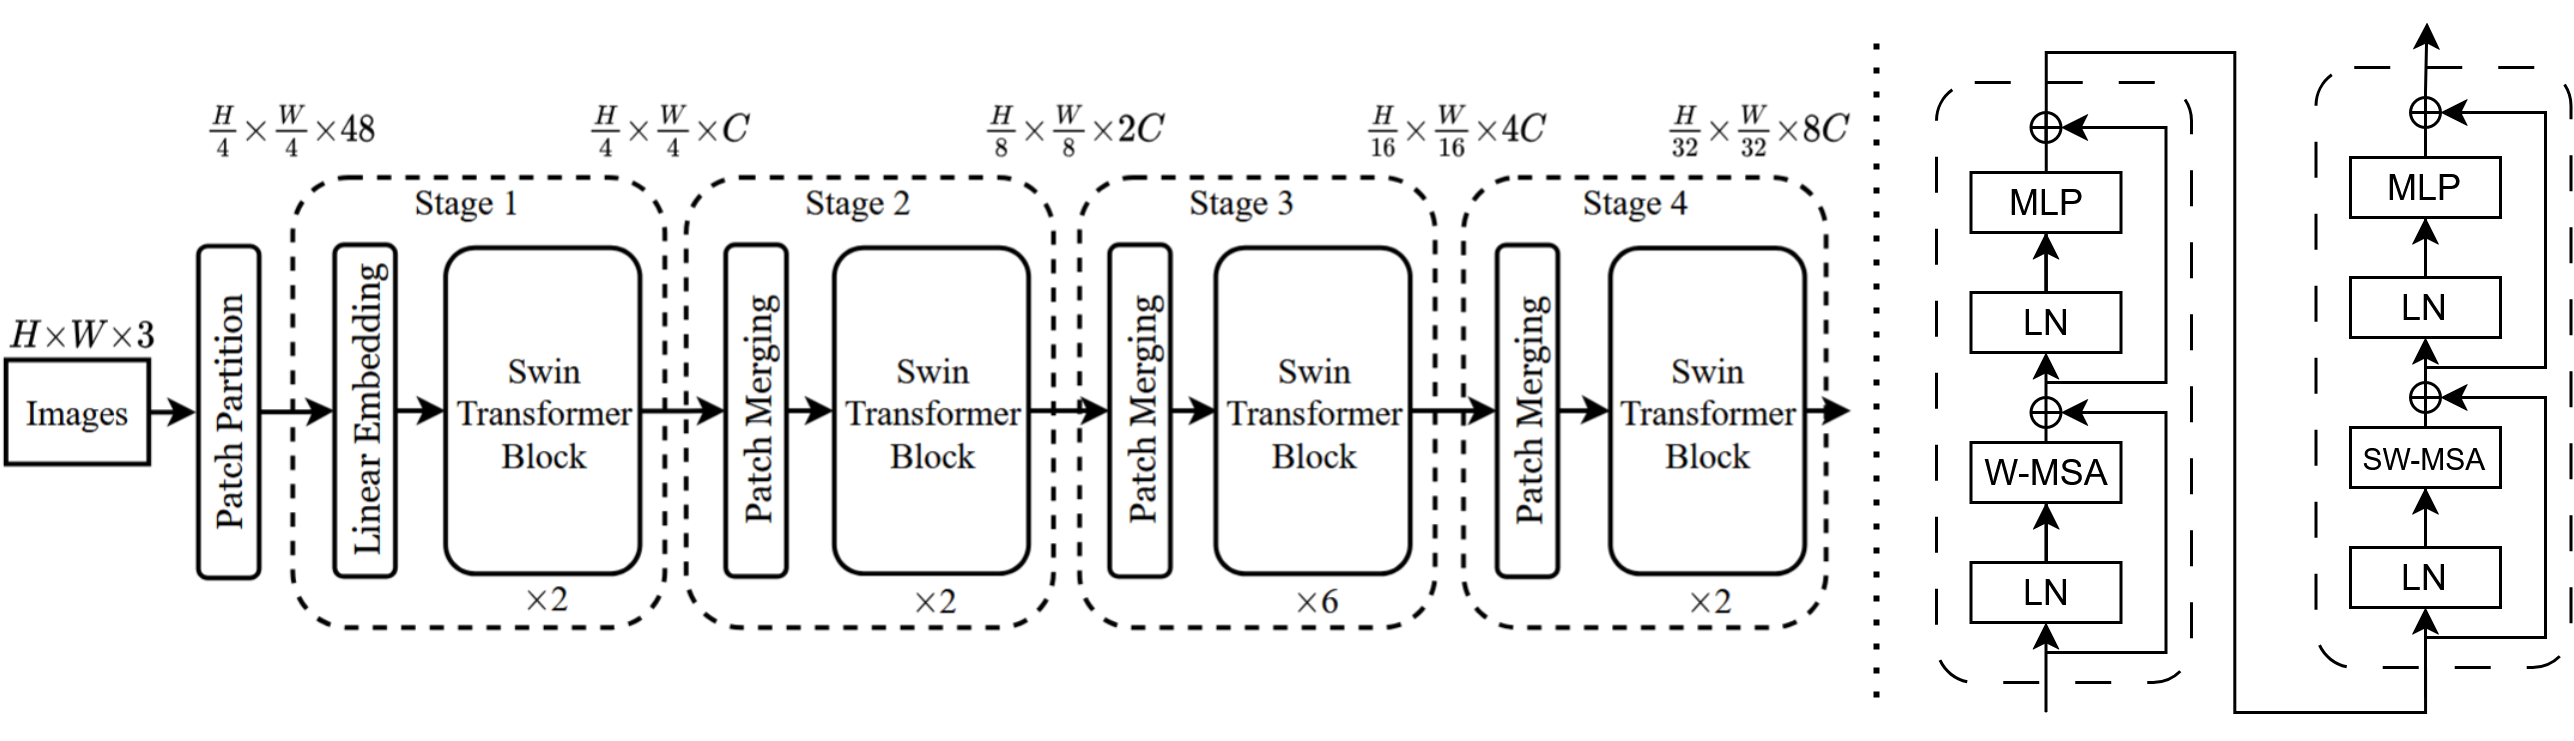
\includegraphics[width=1\textwidth]{images/swin-architecture.png}
    \caption{Arsitektur dan cara kerja \swin{} \parencite{liu2021swin}.}
    \label{fig:swin-architecture}
\end{figure}

\swin{} menggunakan \emph{Window Multi-Head Self-Attention} (W-MSA). Dengan metode ini, mekanisme \selfattention{} hanya dilakukan dalam \emph{window} lokal yang \emph{non-overlapping}. Contohnya ditunjukkan pada \autoref{fig:Swin-shifted-window}. 
Setiap \emph{window} memiliki ukuran $M \times M$ (umumnya $7 \times 7$) dan dengan membatasi \emph{attention} pada setiap \emph{window}, kompleksitas komputasi berkurang dari kuadratik menjadi linear terhadap ukuran gambar.

Untuk memungkinkan koneksi \emph{cross-window}, \swin{} 
menggunakan metode \emph{Shifted Window Multi-Head Self-Attention} (SW-MSA). 
Dalam metode ini, setiap window akan bergeser pada lapisan berikutnya dengan jarak tertentu (misalnya setengah ukuran jendela). Ini menciptakan koneksi cross window tanpa menambah banyak beban komputasi. Proses ini dapat dilihat pada \autoref{fig:Swin-shifted-window}. Window pada lapisan $l$ dan $l+1$ digeser untuk menciptakan interaksi 
satu sama lain. Dalam proses self-attention, Swin Transformer menggunakan \textit{relative position bias} untuk menangkap hubungan spasial antar \patch{}.


\subsection{\bartfull}
\label{subsec:bart}

\bartfull adalah adalah model \ml{} yang dirancang untuk memahami, menghasilkan, dan merekonstruksi teks dalam bahasa alami (\emph{natural language}). \bart{} merupakan \emph{denoising autoencoder} yang dilatih untuk memperbaiki teks yang telah "dirusak" (di-\emph{noise}) oleh berbagai transformasi sehingga mampu mengembalikan teks ke bentuk aslinya \parencite{lewis2019bart}. Arsitektur \bart{} menggabungkan kelebihan model \bert{} yang memiliki \emph{encoder bidirectional} dan GPT yang menggunakan \emph{decoder autoregressive}. Hal ini menjadikannya sangat fleksibel untuk berbagai tugas \nlpfull.

\bart{} dibangun di atas arsitektur transformer yang terdiri atas dua 
komponen utama, yaitu \emph{bidirectional encoder} dan \textit{autoregressive decoder}. 
\emph{Bidirectional encoder} akan mengolah teks input dengan cara memahami hubungan antar token secara dua arah. \emph{Autoregressive decoder} akan menghasilkan teks secara berurutan, token demi token, dengan mempertimbangkan \emph{sequence} yang sudah dihasilkan.

\begin{figure}
\centering
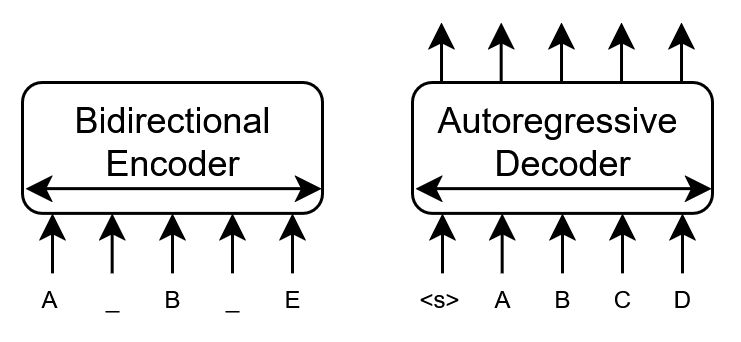
\includegraphics[width=0.8\textwidth]{images/bart.png}
\caption{Cara kerja \bart{} \parencite{lewis2019bart}.}
\label{fig:bart}
\end{figure}

\autoref{fig:bart} menunjukkan cara \bart{} bekerja. Teks input akan “dirusak” terlebih dahulu, kemudian dibaca oleh \encoder. Hasil bacaan \encoder{} akan diteruskan ke \decoder{} untuk mengembalikan bagian teks yang “dirusak” secara 
\textit{autoregressive}. Dengan kemampuannya untuk merekonstruksi teks dari masukan yang rusak, \bart{} menjadi suatu \transformer{} yang sangat baik untuk memahami struktur bahasa dan menghasilkan teks yang koheren walaupun masukan dinilai 
rusak. Penggunaan \bart{} mirip dengan \bert{} dan GPT, seperti klasifikasi teks, generasi teks, dan penejermahan teks. 




